\section{Datasets}

All data comes from Hugging Face, which is on the department's approved list; Kaggle was not used. Table~\ref{tab:data} lists the three evaluation sets.

\begin{itemize}
	\item \textbf{Spider} \cite{yu2018spider}, the benchmark on which CodeS reports its results: questions, gold SQL and SQLite databases, with training and development sets on disjoint databases, so a model is always evaluated on schemas it has never seen. Questions from \path{xlangai/spider} (the authors' organisation), databases from \path{HAL-9001/spider-databases}.
	\item \textbf{Spider-Realistic} \cite{deng2020structuregrounded}: 508 Spider development questions rewritten by their authors so that they no longer name the columns (``from the oldest to the youngest'' instead of ``ordered by age''), with the same databases and gold SQL; from \path{aherntech/spider-realistic} (a copy of the authors' release, CC BY-SA 4.0).
	\item \textbf{BIRD Mini-Dev} \cite{li2023can}: the BIRD authors' 500-question subset over 11 real-world databases (finance, medicine, sport, schools and others) of up to 571\,MB, with dirty values and an expert ``evidence'' hint per question; questions from the official \path{birdsql/bird_mini_dev}, databases from \path{nlile/BIRD-bench}.
\end{itemize}

\begin{table}[!t]
	\centering
	\caption{Evaluation sets.}
	\label{tab:data}
	\singlespacing
	\begin{tabular}{|l|r|r|l|}
		\hline
		\textbf{Set} & \textbf{Questions} & \textbf{Databases} & \textbf{Used for} \\ \hline
		Spider development & 1,034 & 20 & Reproduction, ablation, enhancement \\ \hline
		Spider-Realistic & 508 & 19 & Realistic wording \\ \hline
		BIRD Mini-Dev & 500 & 11 & Real-world databases \\ \hline
	\end{tabular}
\end{table}

The Spider development databases are small: 2 to 11 tables (4.05 on average) and 7 to 56 columns. Of the 1,034 gold queries, 39.5\% need a join, 26.8\% a \texttt{GROUP BY}, 8.0\% a nested query and 7.7\% a set operation --- the constructs where a query can run without error and still return the wrong rows. By the official difficulty classifier, 248 questions are easy, 446 medium, 174 hard and 166 extra hard.

\section{Architecture}

Figure~\ref{fig:pipeline} shows the system. The reproduced CodeS components build the database prompt, generate four candidate queries and select one. The enhancement executes all four candidates, measures how many return the same result and decides whether to answer or to ask the user. The application wraps this pipeline in a desktop interface, and the evaluation and the application run the same code.

\begin{figure}[!t]
	\centering
	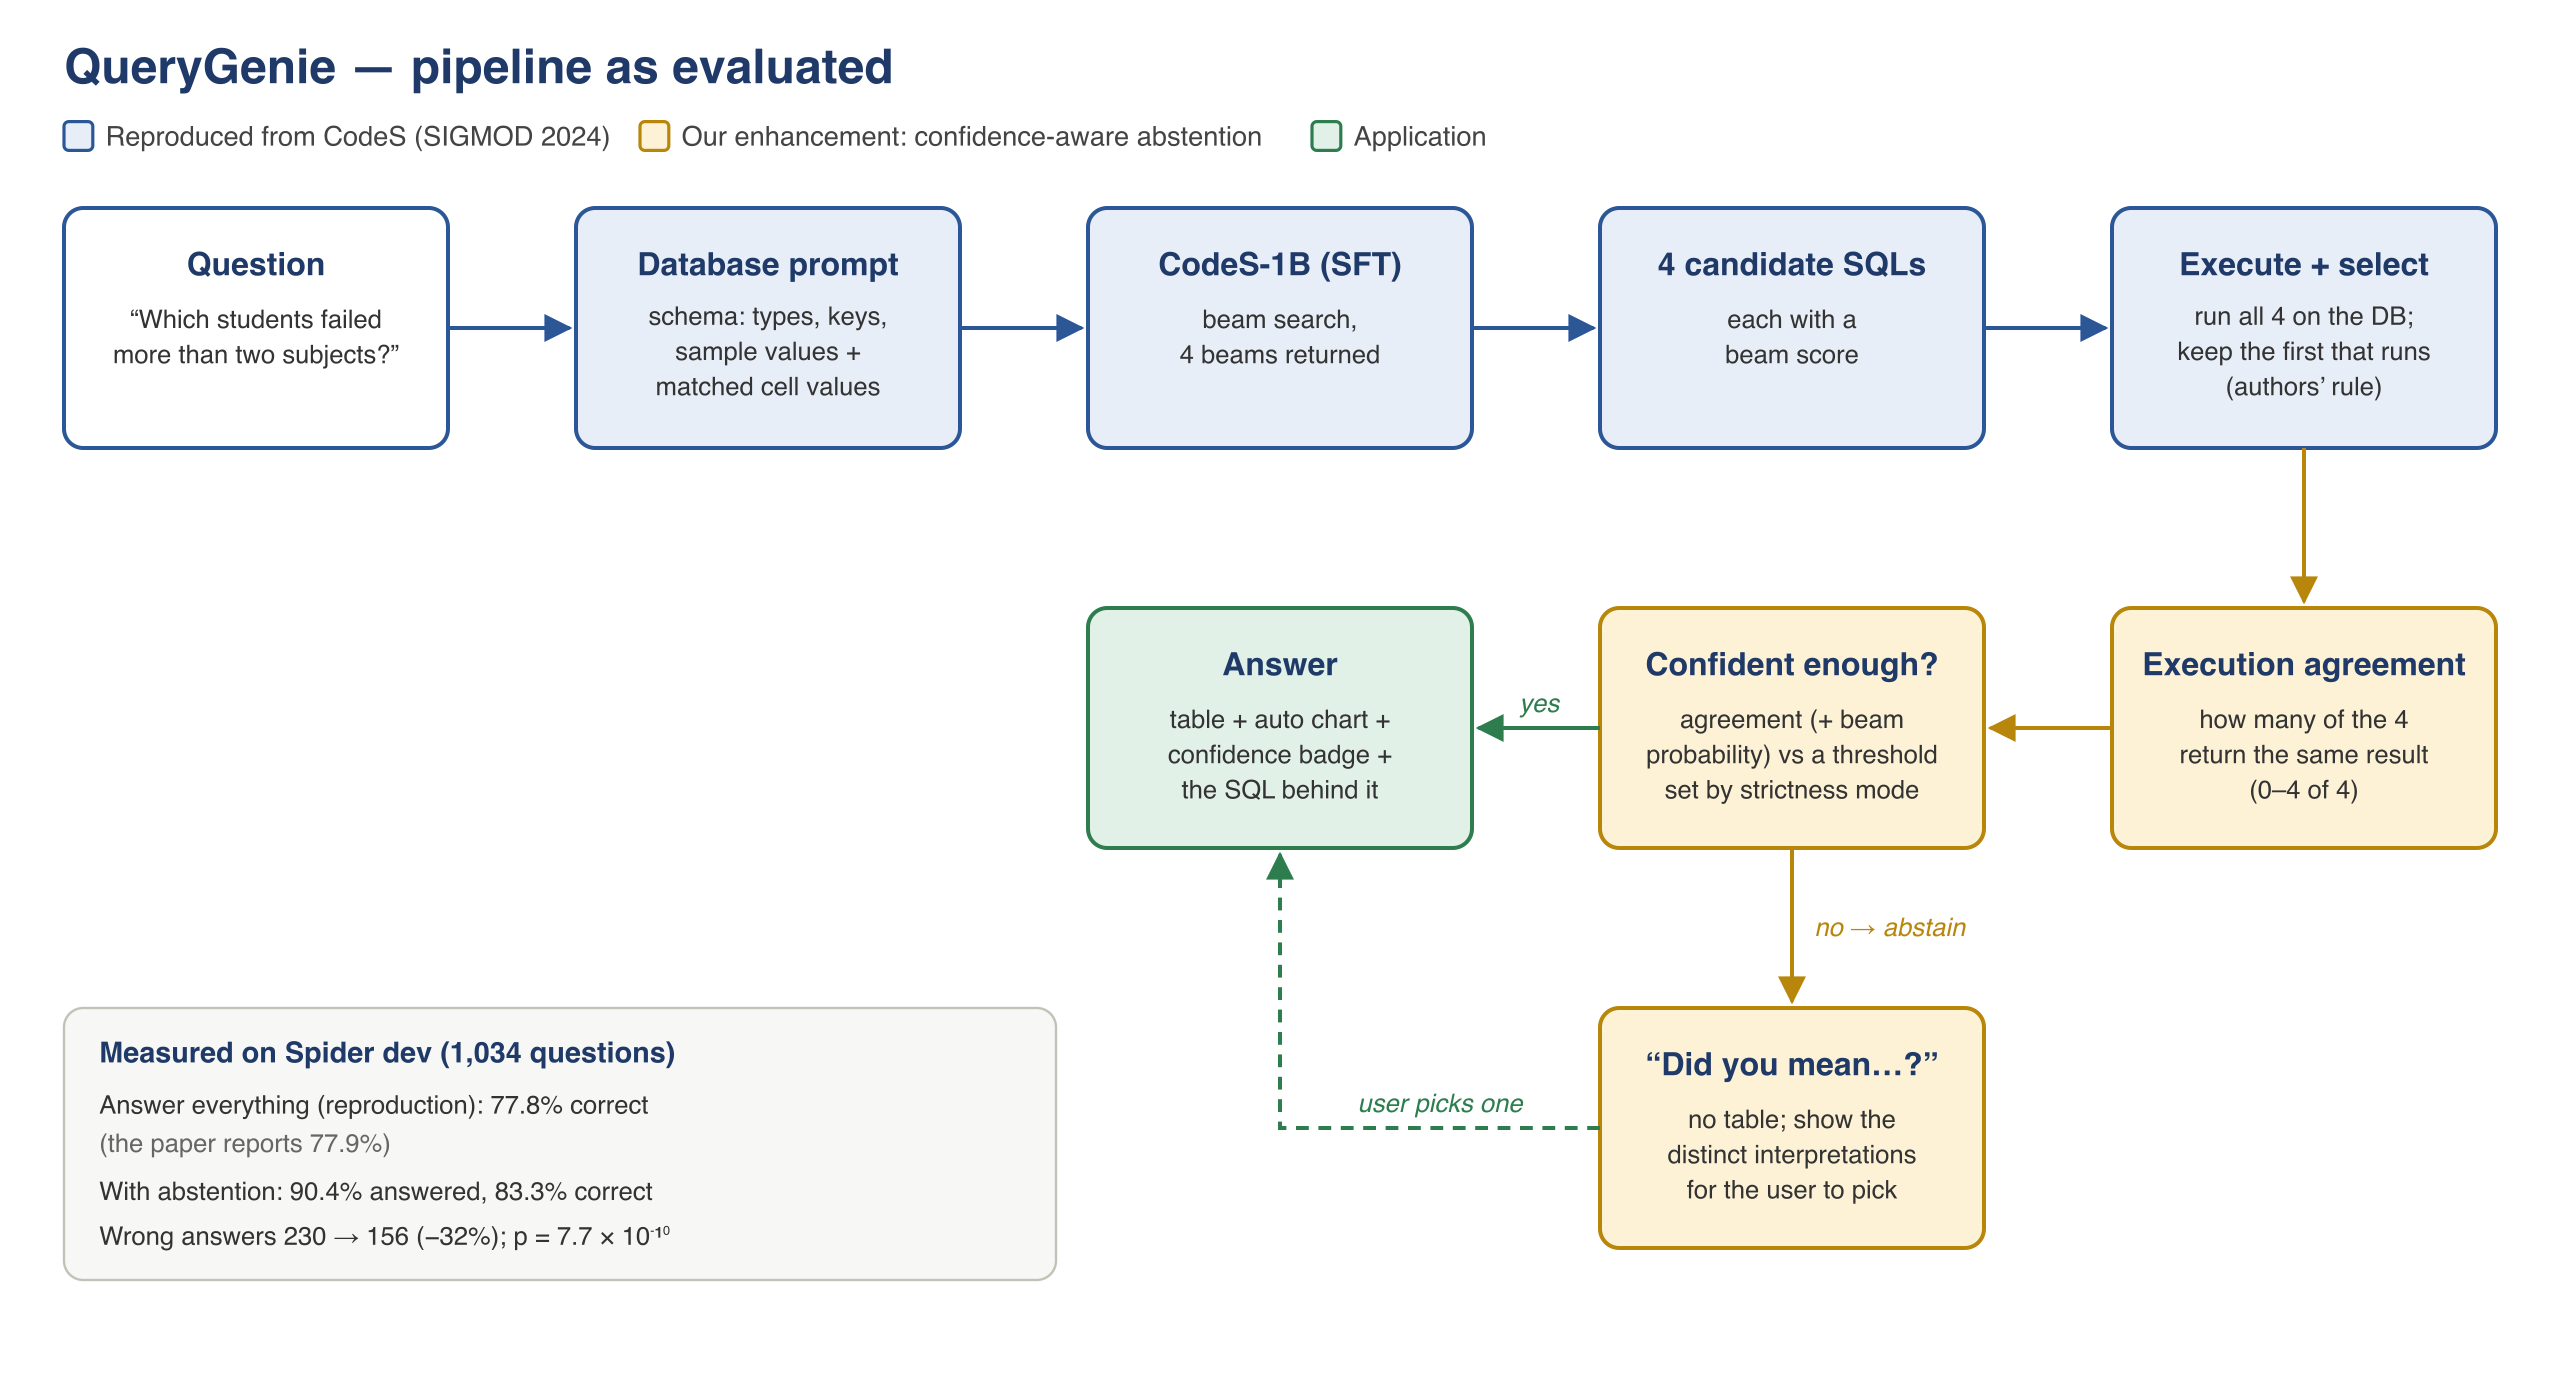
\includegraphics[width=\linewidth]{images/figures/final_pipeline.png}
	\caption{System architecture: reproduced CodeS components (blue), the enhancement (amber) and the application (green).}
	\label{fig:pipeline}
\end{figure}

\section{The reproduced CodeS pipeline}

CodeS does not see the raw database. For each question it builds a textual prompt, exactly as in the authors' code (Figure~\ref{fig:codes}):

\begin{itemize}
	\item \textbf{Schema sequence:} every table with its columns, types, primary keys, foreign keys and a few representative values per column.
	\item \textbf{Column descriptions:} human-readable names from the dataset's schema file, where they differ from the column name.
	\item \textbf{Matched contents:} stored values that match words in the question, found by the authors' value retriever (string similarity of at least 0.9, at most 25 values per column).
\end{itemize}

The question follows, and the model generates four candidates with beam search. The first candidate that SQLite accepts (\texttt{EXPLAIN QUERY PLAN}) is returned, otherwise the first beam --- the rule in the authors' inference code. Prompts longer than 3,840 tokens are cut from the start, as the authors do; no Spider prompt is that long.

\begin{figure}[!t]
	\centering
	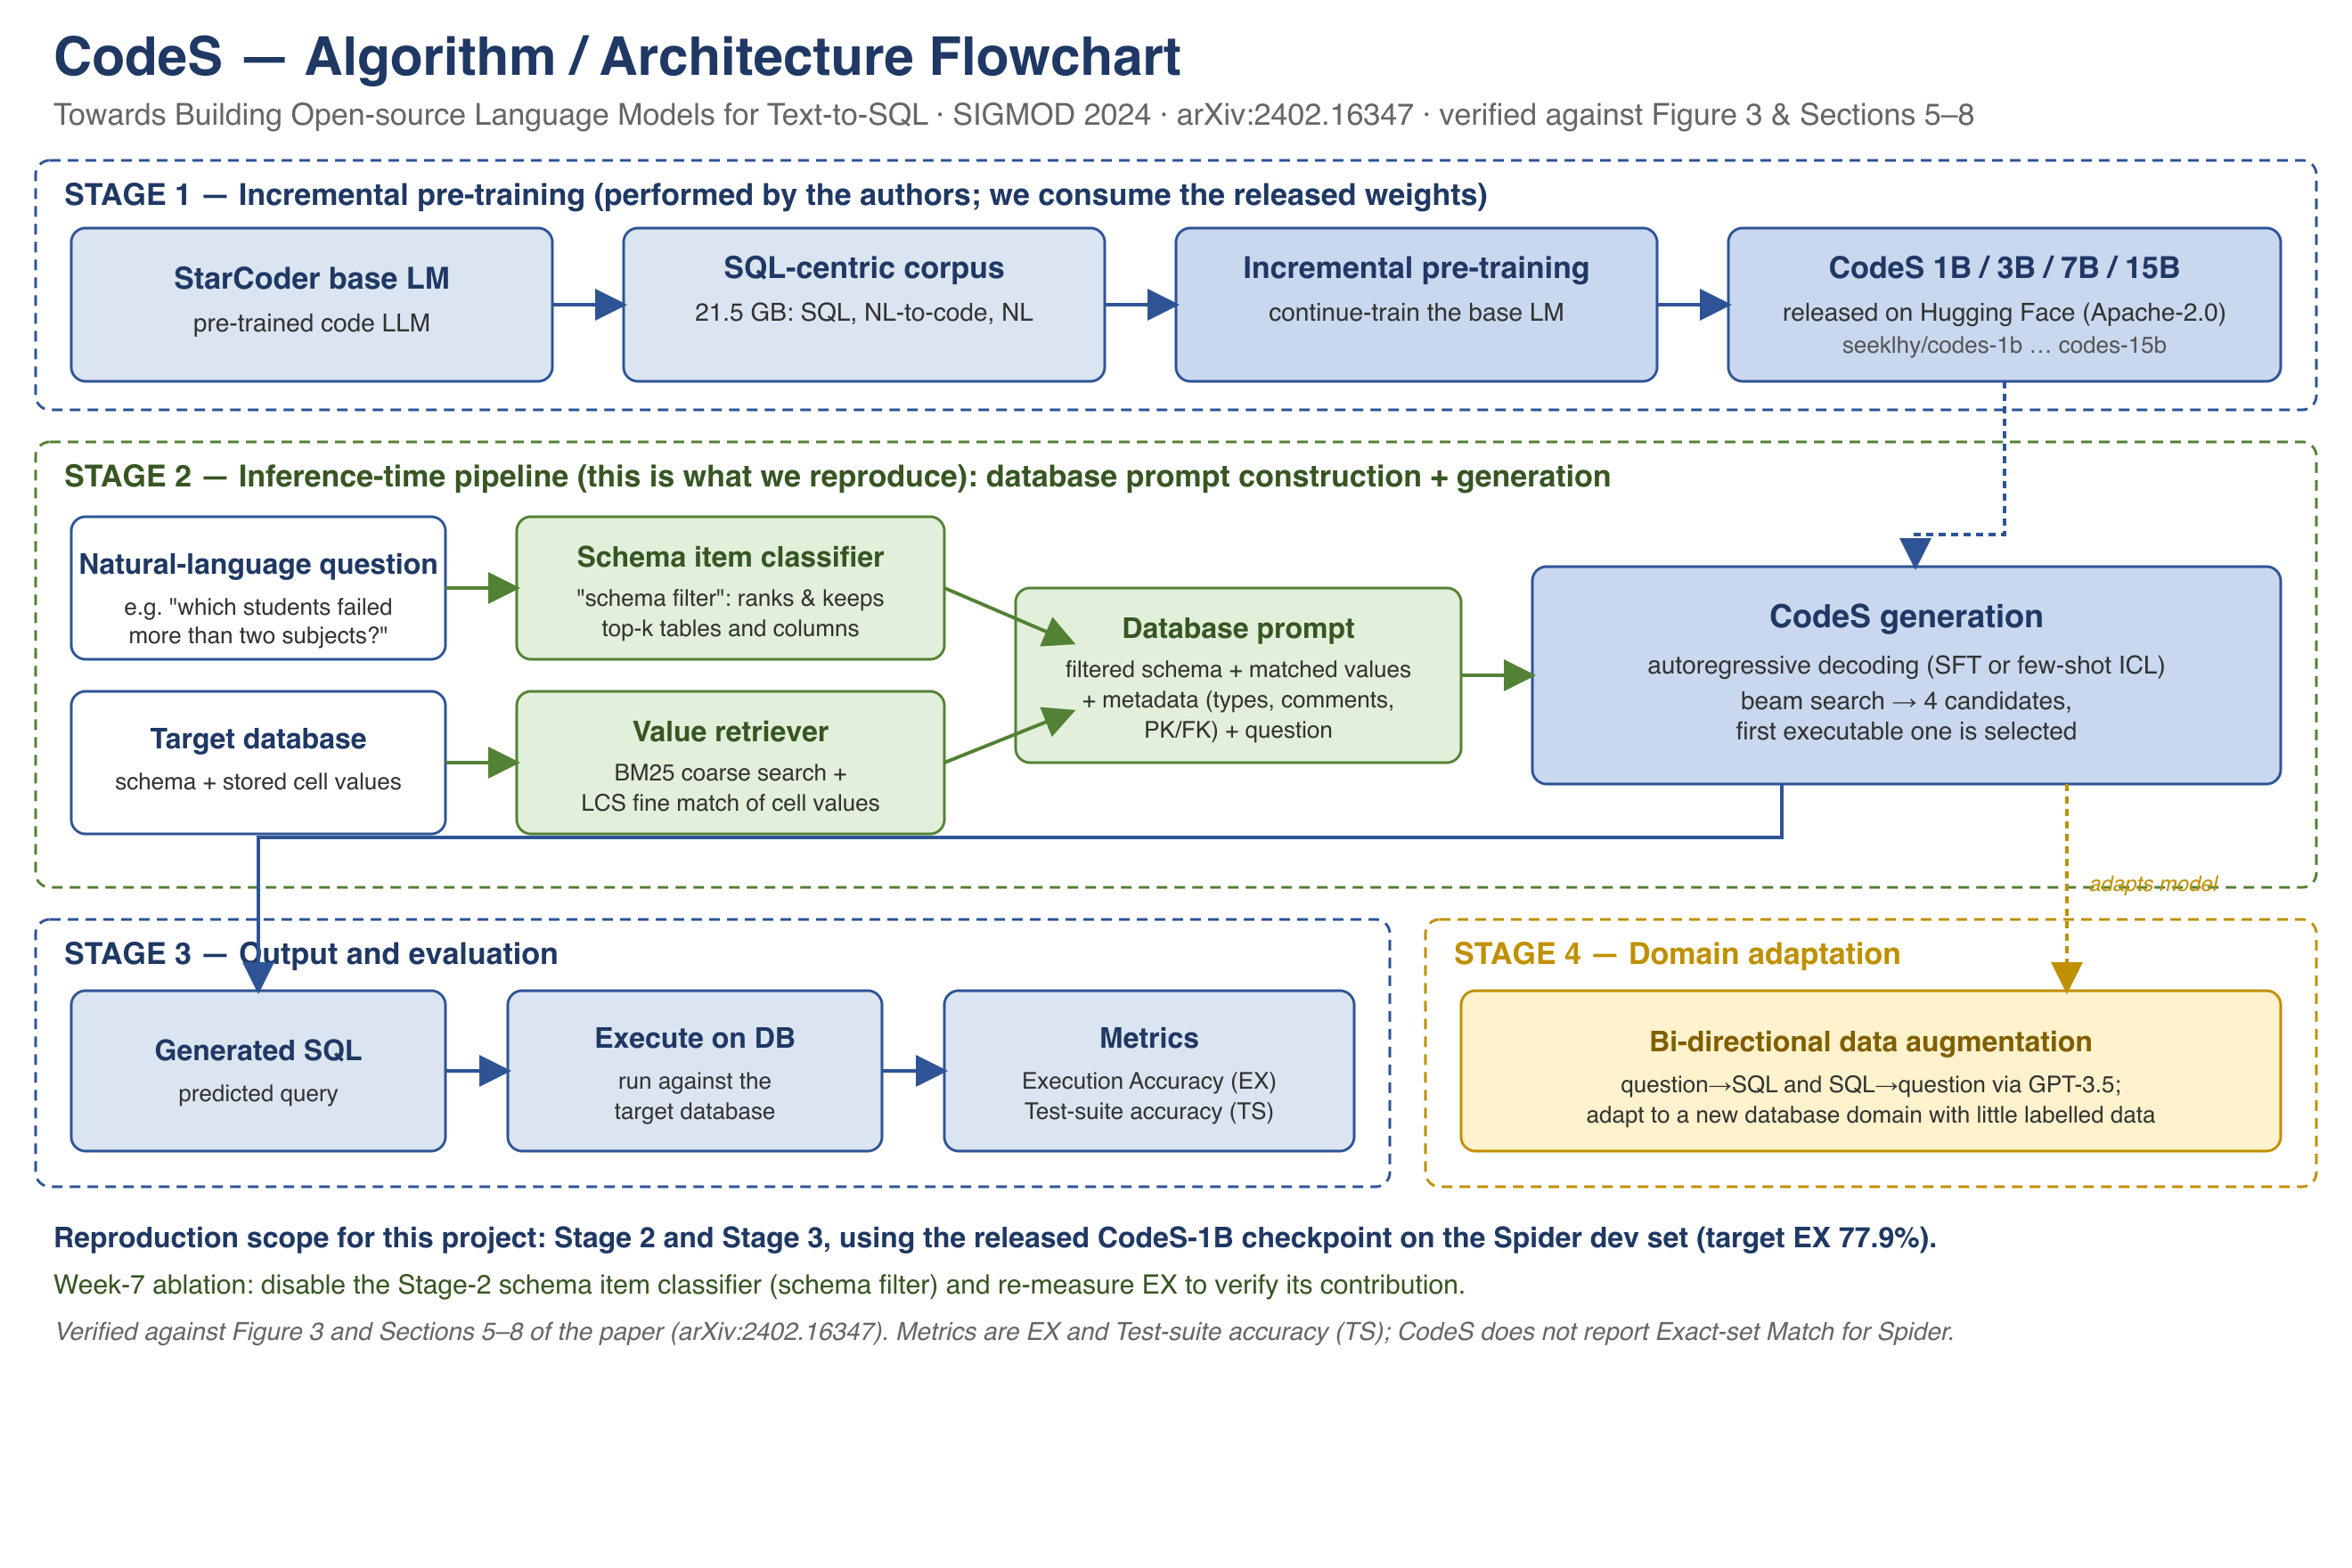
\includegraphics[width=0.85\linewidth]{images/figures/codes_architecture_flowchart.png}
	\caption{The CodeS pipeline, annotated from the paper.}
	\label{fig:codes}
\end{figure}

\textbf{Environment and harness.} The authors used eight NVIDIA A800 GPUs; we used a Tesla T4 (Google Colab, fp16, batch size 1, as in their inference) and an Apple M4 for the realistic evaluations, with newer PyTorch and transformers versions. The reproduction passed the department's Week-4 gate (run T1-001). After early runs scored 64.8--73.8\%, the harness was audited line by line against the authors' code, which found a value-retriever bug (numbers were never matched, changing the prompt for 12.4\% of questions), a simplified scoring metric, missing column descriptions, and predictions that were not saved. All four were fixed; every run since is scored with the official evaluator \cite{zhong2020semantic} and logged with seed, hardware and runtime, including failed and superseded runs.

\textbf{Deviations.} Values are matched by scanning all distinct values instead of the authors' Lucene BM25 pre-filter (no Java dependency; on BIRD a Python word index plays the pre-filter's role); the optional schema classifier is not applied (its checkpoints were unavailable; Spider schemas are small); and test-suite accuracy is TBD, because the distilled test-suite databases were not obtained.

\section{Proposed approach: confidence-aware abstention}

The Week-1 abstract named execution-guided self-correction (DIN-SQL \cite{pourreza2023dinsql}) as the enhancement. The reproduction showed that 97.3\% of CodeS's queries already run, so repairing failures could recover at most 2.7 points, while the dominant error is a query that runs but returns the wrong rows. The enhancement therefore became confidence-aware abstention, combining self-consistency \cite{wang2022selfconsistency} with selective classification \cite{geifman2017selective}; self-correction was kept as an application feature and measured separately (Chapter~4).

All four beam candidates are executed. The confidence of the returned answer is the share of candidates whose result equals it --- execution agreement, from 0 to 4 of 4, and zero when the returned query does not run --- with the beam probability used only to break ties. Below a threshold $\tau$ the system abstains: it shows no table and offers the distinct results of the candidates as readings for the user to choose from (Algorithm~\ref{alg:abstain}). No retraining is involved.

\begin{algorithm}[!t]
	\SetAlgoLined
	\KwIn{question $Q$, database $D$, threshold $\tau$}
	\KwOut{an answer, or the readings for the user to choose from}
	$P \leftarrow$ CodeS database prompt for $(Q, D)$\;
	$(s_1, \dots, s_4), (b_1, \dots, b_4) \leftarrow$ four beam candidates and their scores\;
	\For{$i \leftarrow 1$ \KwTo $4$}{
		$r_i \leftarrow$ result of executing $s_i$ on $D$ (read-only; empty if it fails)\;
	}
	$k \leftarrow$ first $i$ whose query passes \texttt{EXPLAIN QUERY PLAN}, else $1$\;
	$a \leftarrow \frac{1}{4}\,\lvert\{\, i : r_i = r_k \,\}\rvert$ if $s_k$ runs, else $0$\;
	$c \leftarrow a + 0.01\, e^{b_k} / \sum_j e^{b_j}$\;
	\eIf{$c \ge \tau$}{
		\Return result $r_k$ with agreement $a$\;
	}{
		\Return the distinct results among $r_1, \dots, r_4$ as readings\;
	}
	\caption{Confidence-aware abstention on top of CodeS}
	\label{alg:abstain}
\end{algorithm}

\textbf{Hypothesis and protocol} (fixed before the results were seen). H1: at the same coverage, accuracy on answered questions is higher with agreement-based abstention than with random abstention and than the 77.8\% baseline; H0: no difference. Over 10 random 50/50 splits of the development set, the threshold is set on the calibration half for at least 90\% coverage and applied to the test half; the paired gain is tested with a one-sided paired t-test and a Wilcoxon signed-rank test ($\alpha = 0.05$), and checked with a 5,000-sample bootstrap over questions. The application uses $\tau = 0.2526$, the median of the calibration thresholds: it abstains when no candidate runs, or when only 1 of 4 supports the answer and its beam probability is low.

\section{The application}

QueryGenie is a desktop application for macOS and Windows. A setup assistant downloads the model (about 4.5\,GB) on first start; everything then runs locally on open weights. Questions are asked in chats; every answer shows how many of the four queries agree, the table, an automatic chart, the SQL and all four candidates, and when the candidates disagree it asks which reading was meant (Figure~\ref{fig:app}). A schema map draws the database, and users can open their own SQLite files or connect read-only to PostgreSQL and MySQL. Failed queries are sent back to the model once with the database error (self-correction), and an empty answer that misses a value stored in the database is sent back with that value. Other models (Ollama, cloud services) can be chosen; they get the same agreement check, labelled as not calibrated.

\begin{figure}[!t]
	\centering
	\subfloat[An answer: all four queries agree; table, chart and SQL are one click away.]{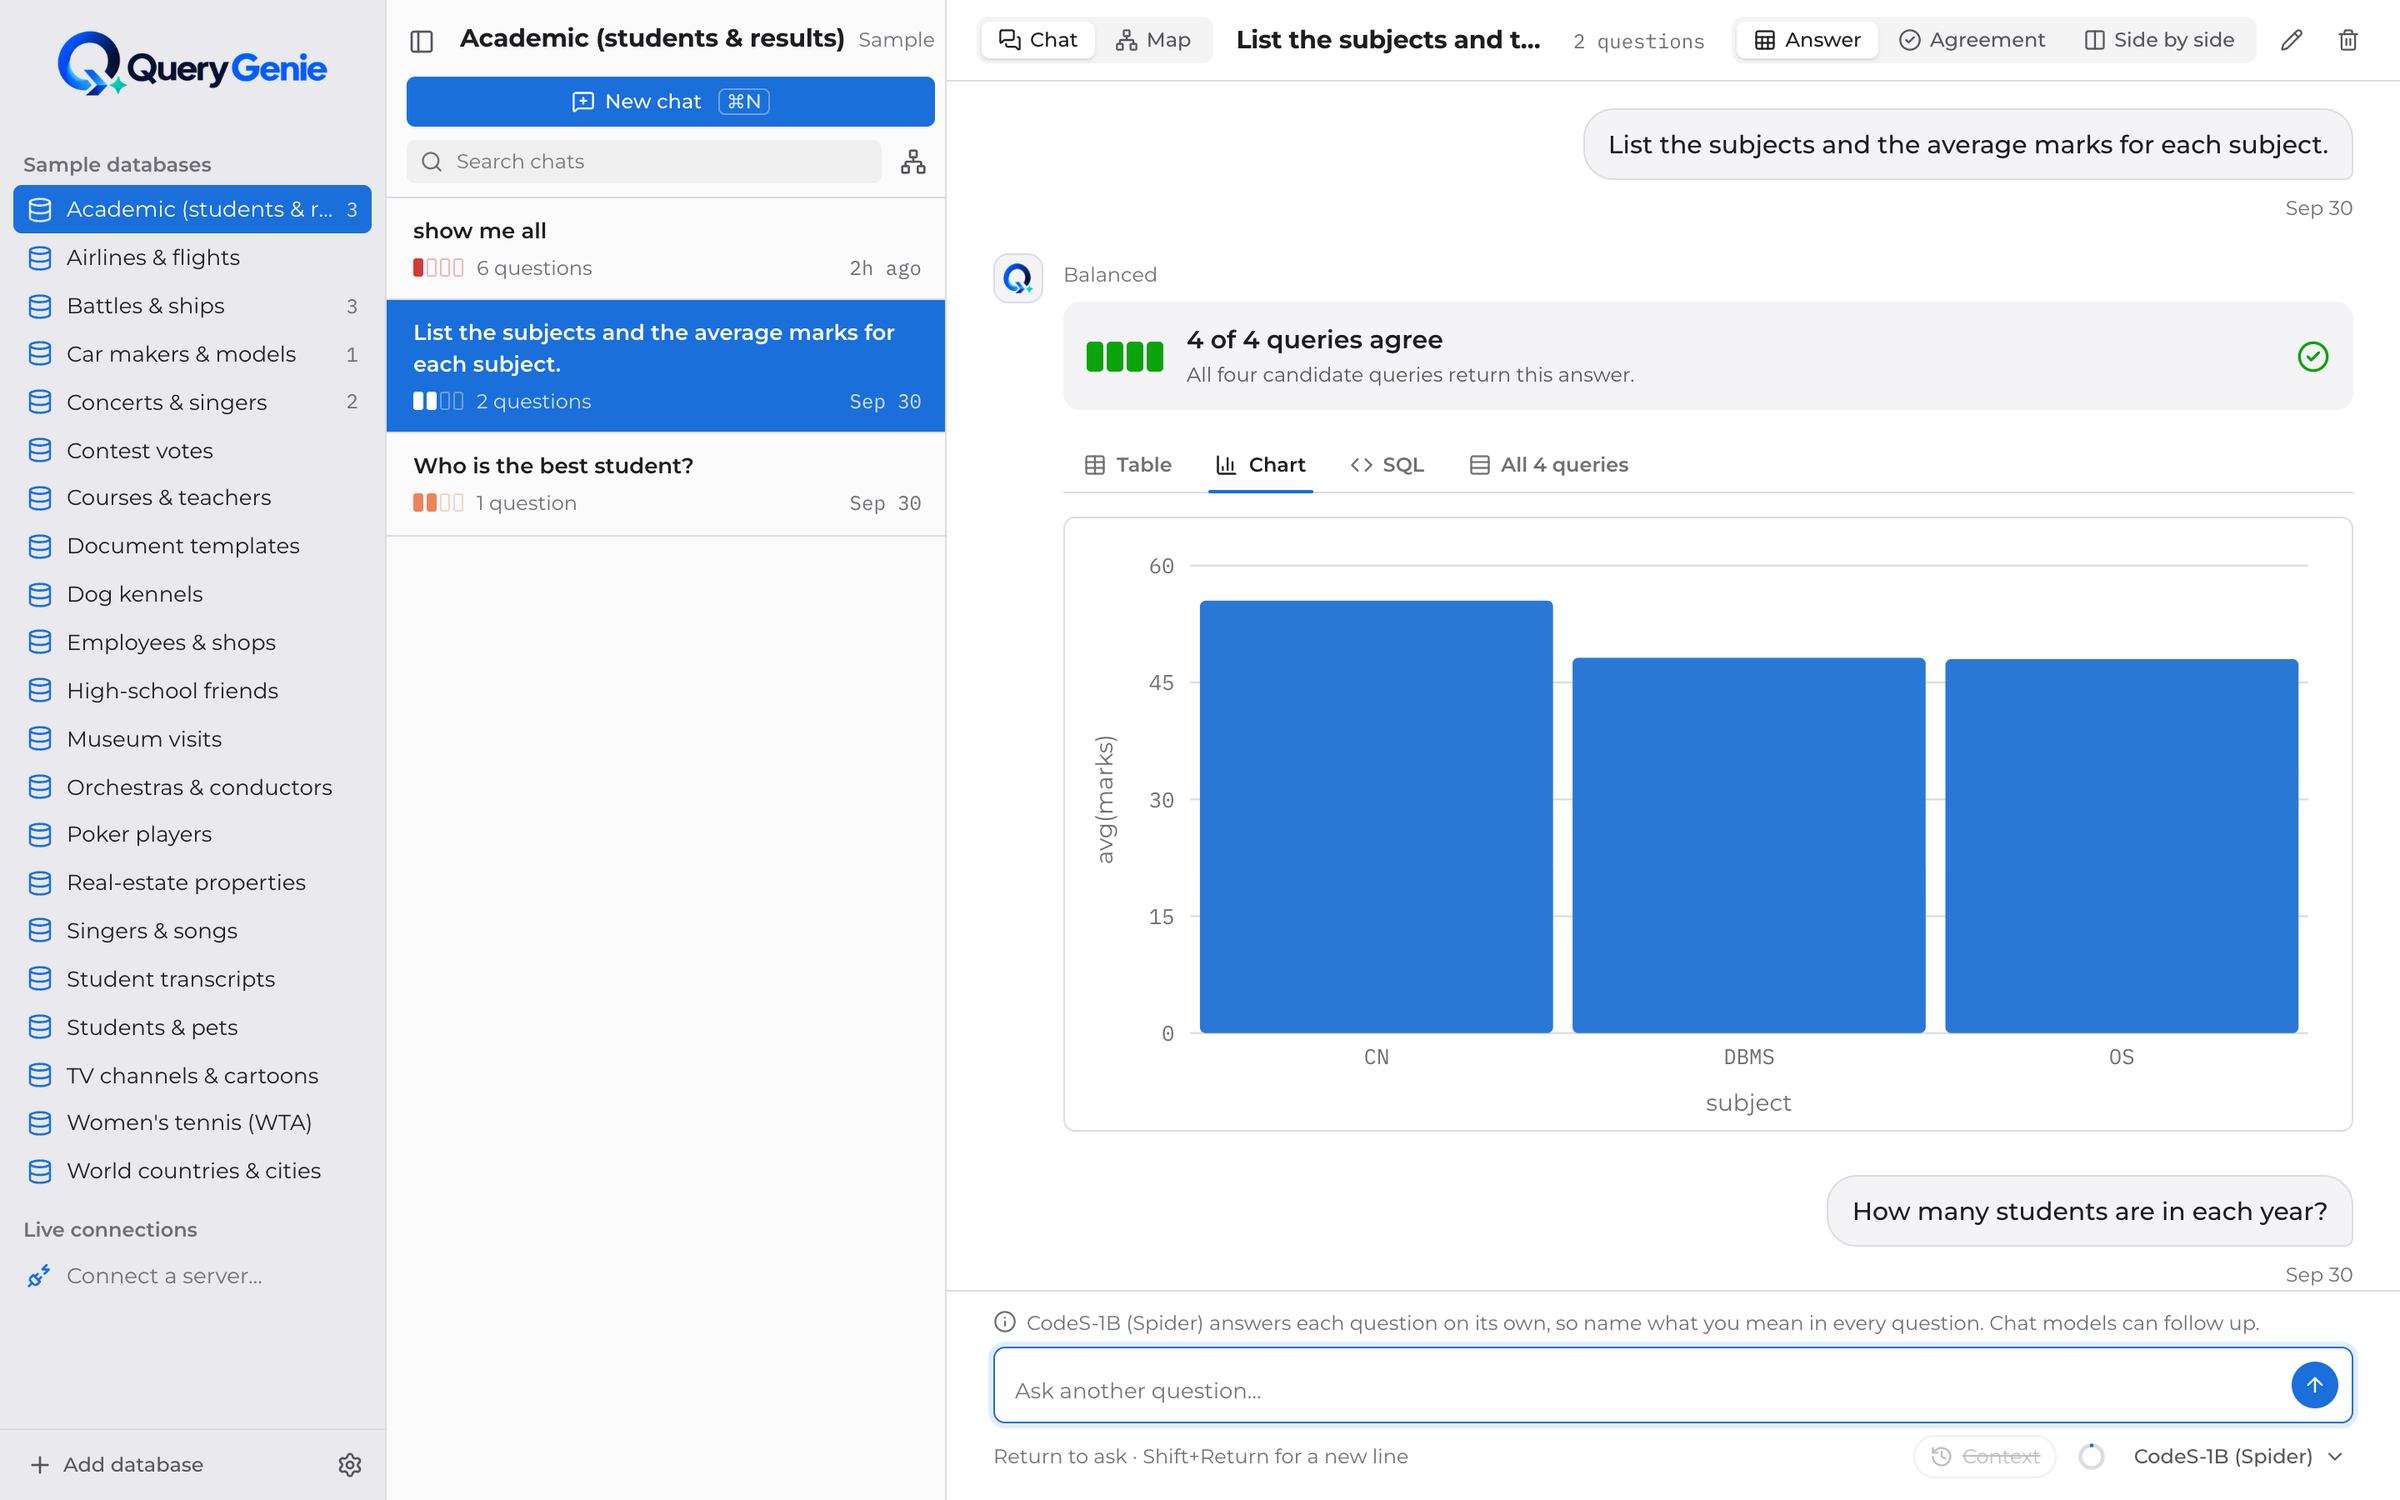
\includegraphics[width=0.49\linewidth]{images/figures/app_answer.png}}\hfill
	\subfloat[Abstention: the queries disagree, so it asks which reading was meant.]{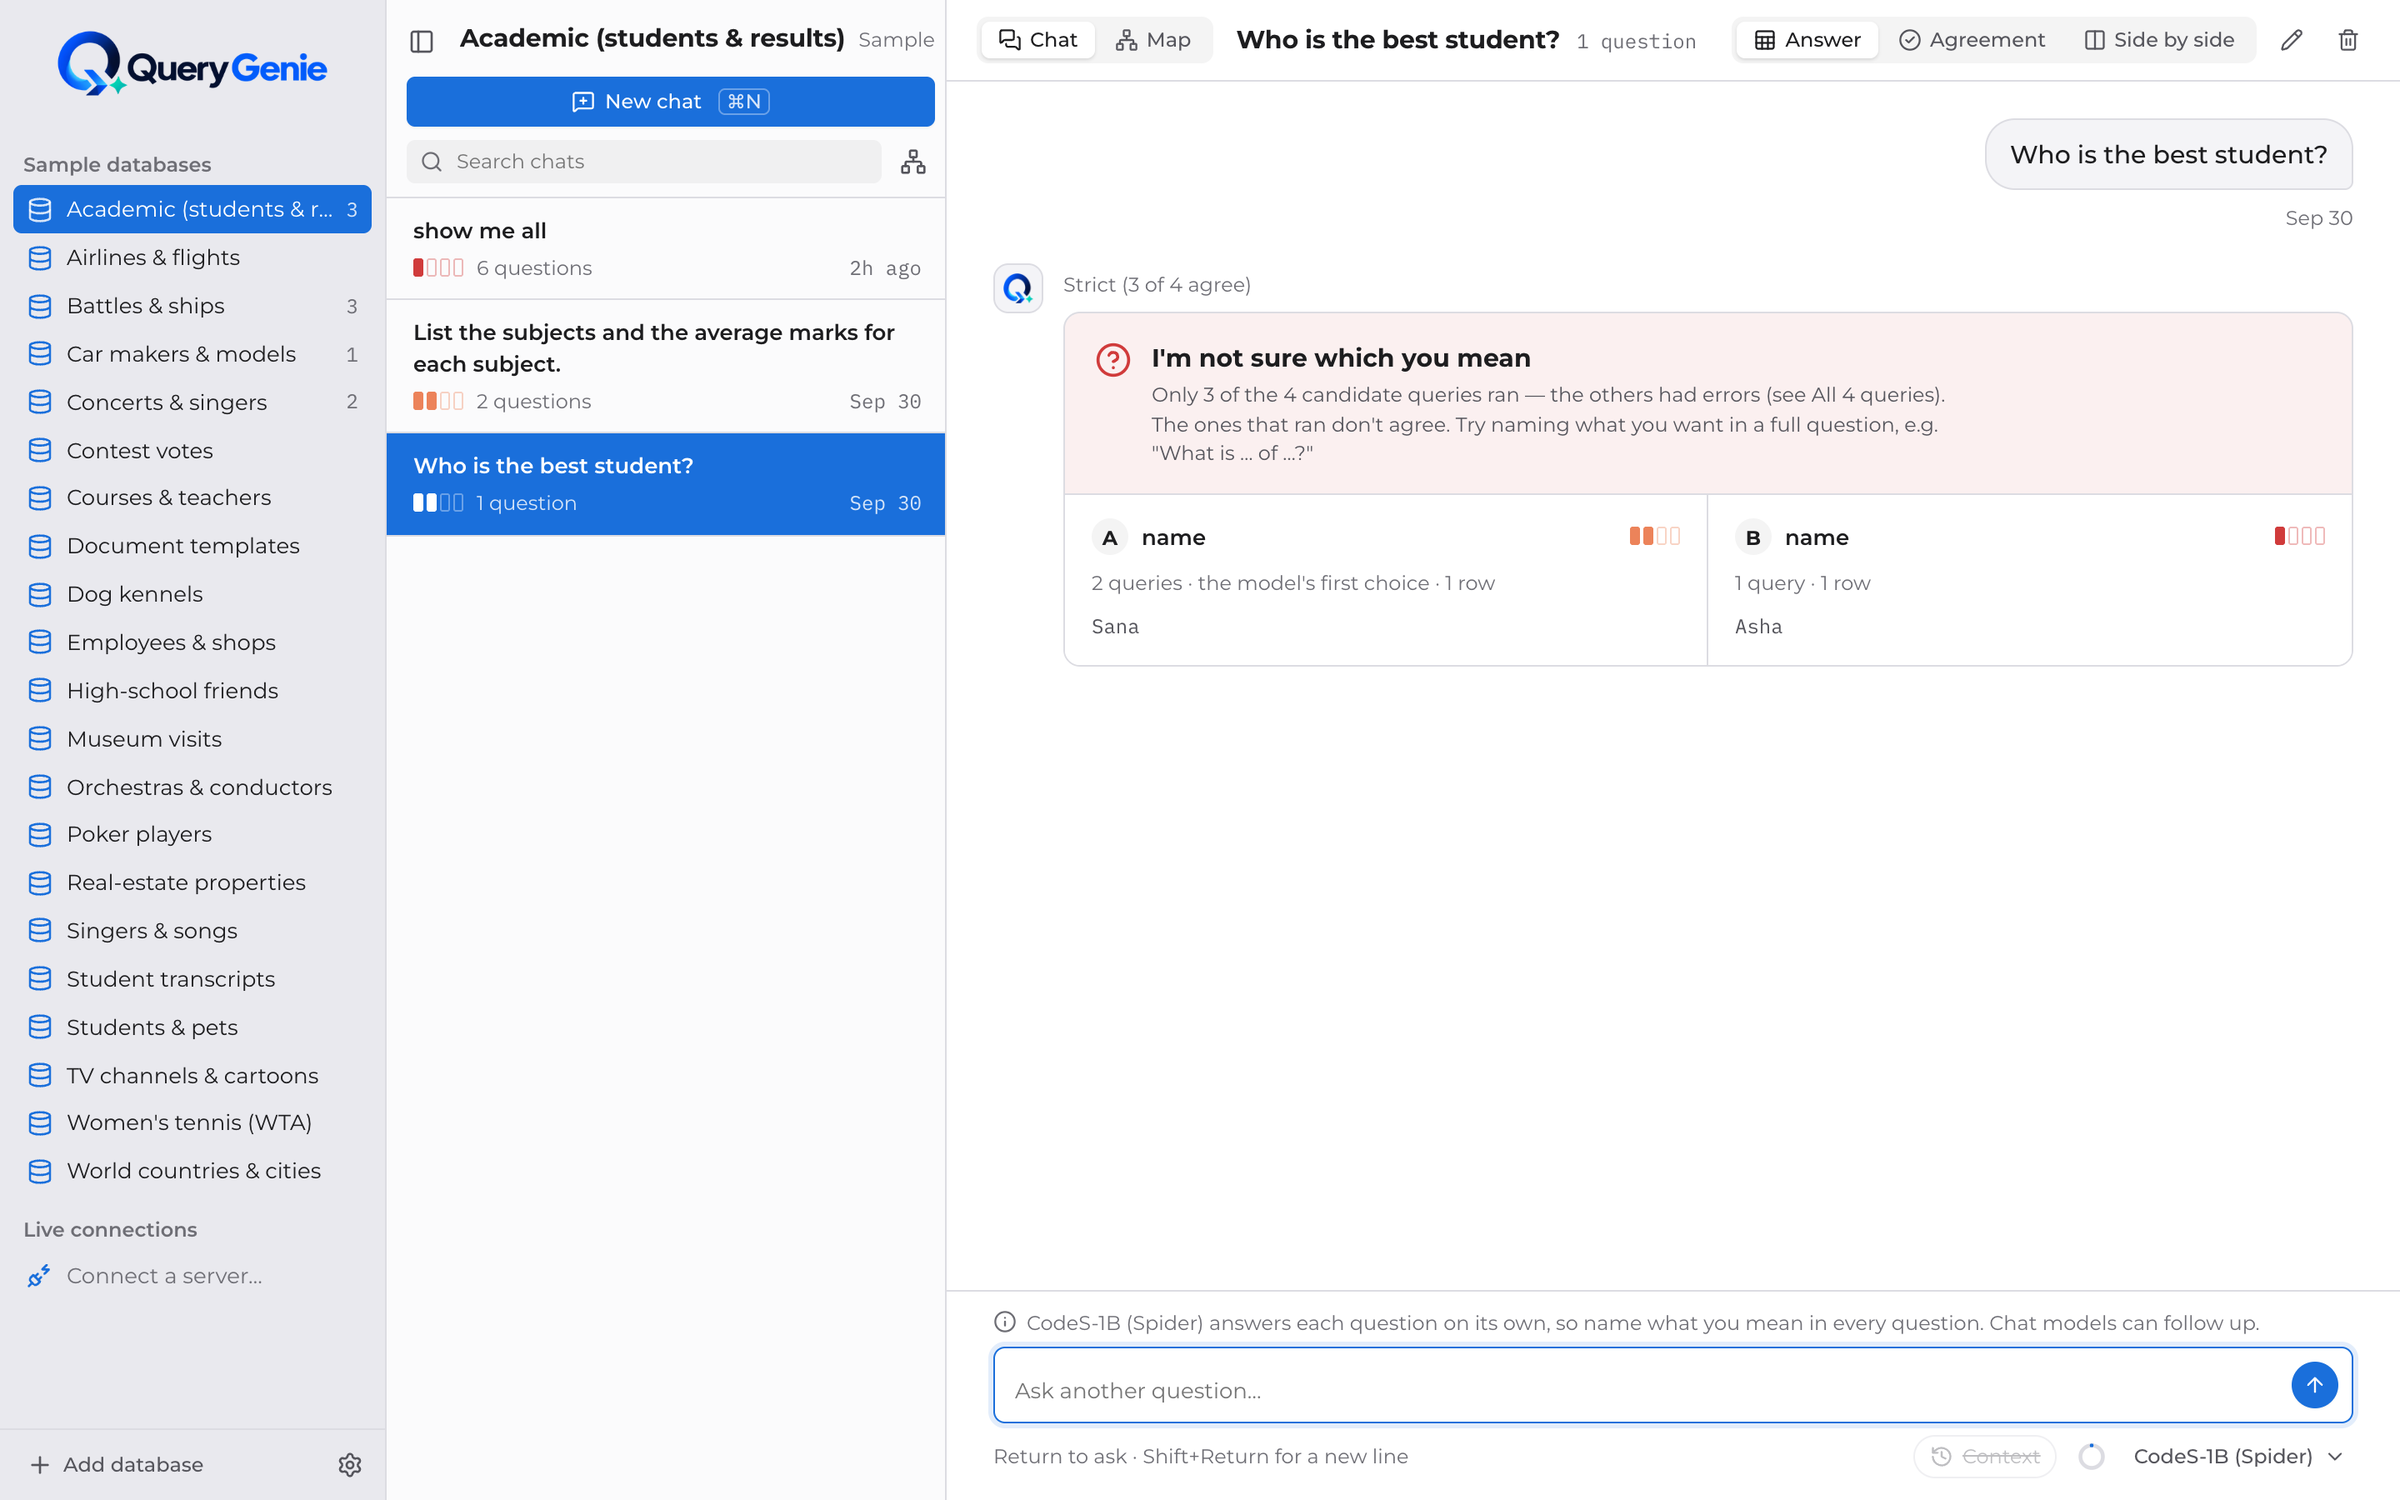
\includegraphics[width=0.49\linewidth]{images/figures/app_not_sure.png}}\\[4pt]
	\subfloat[The schema map: tap a table or column to ask about it.]{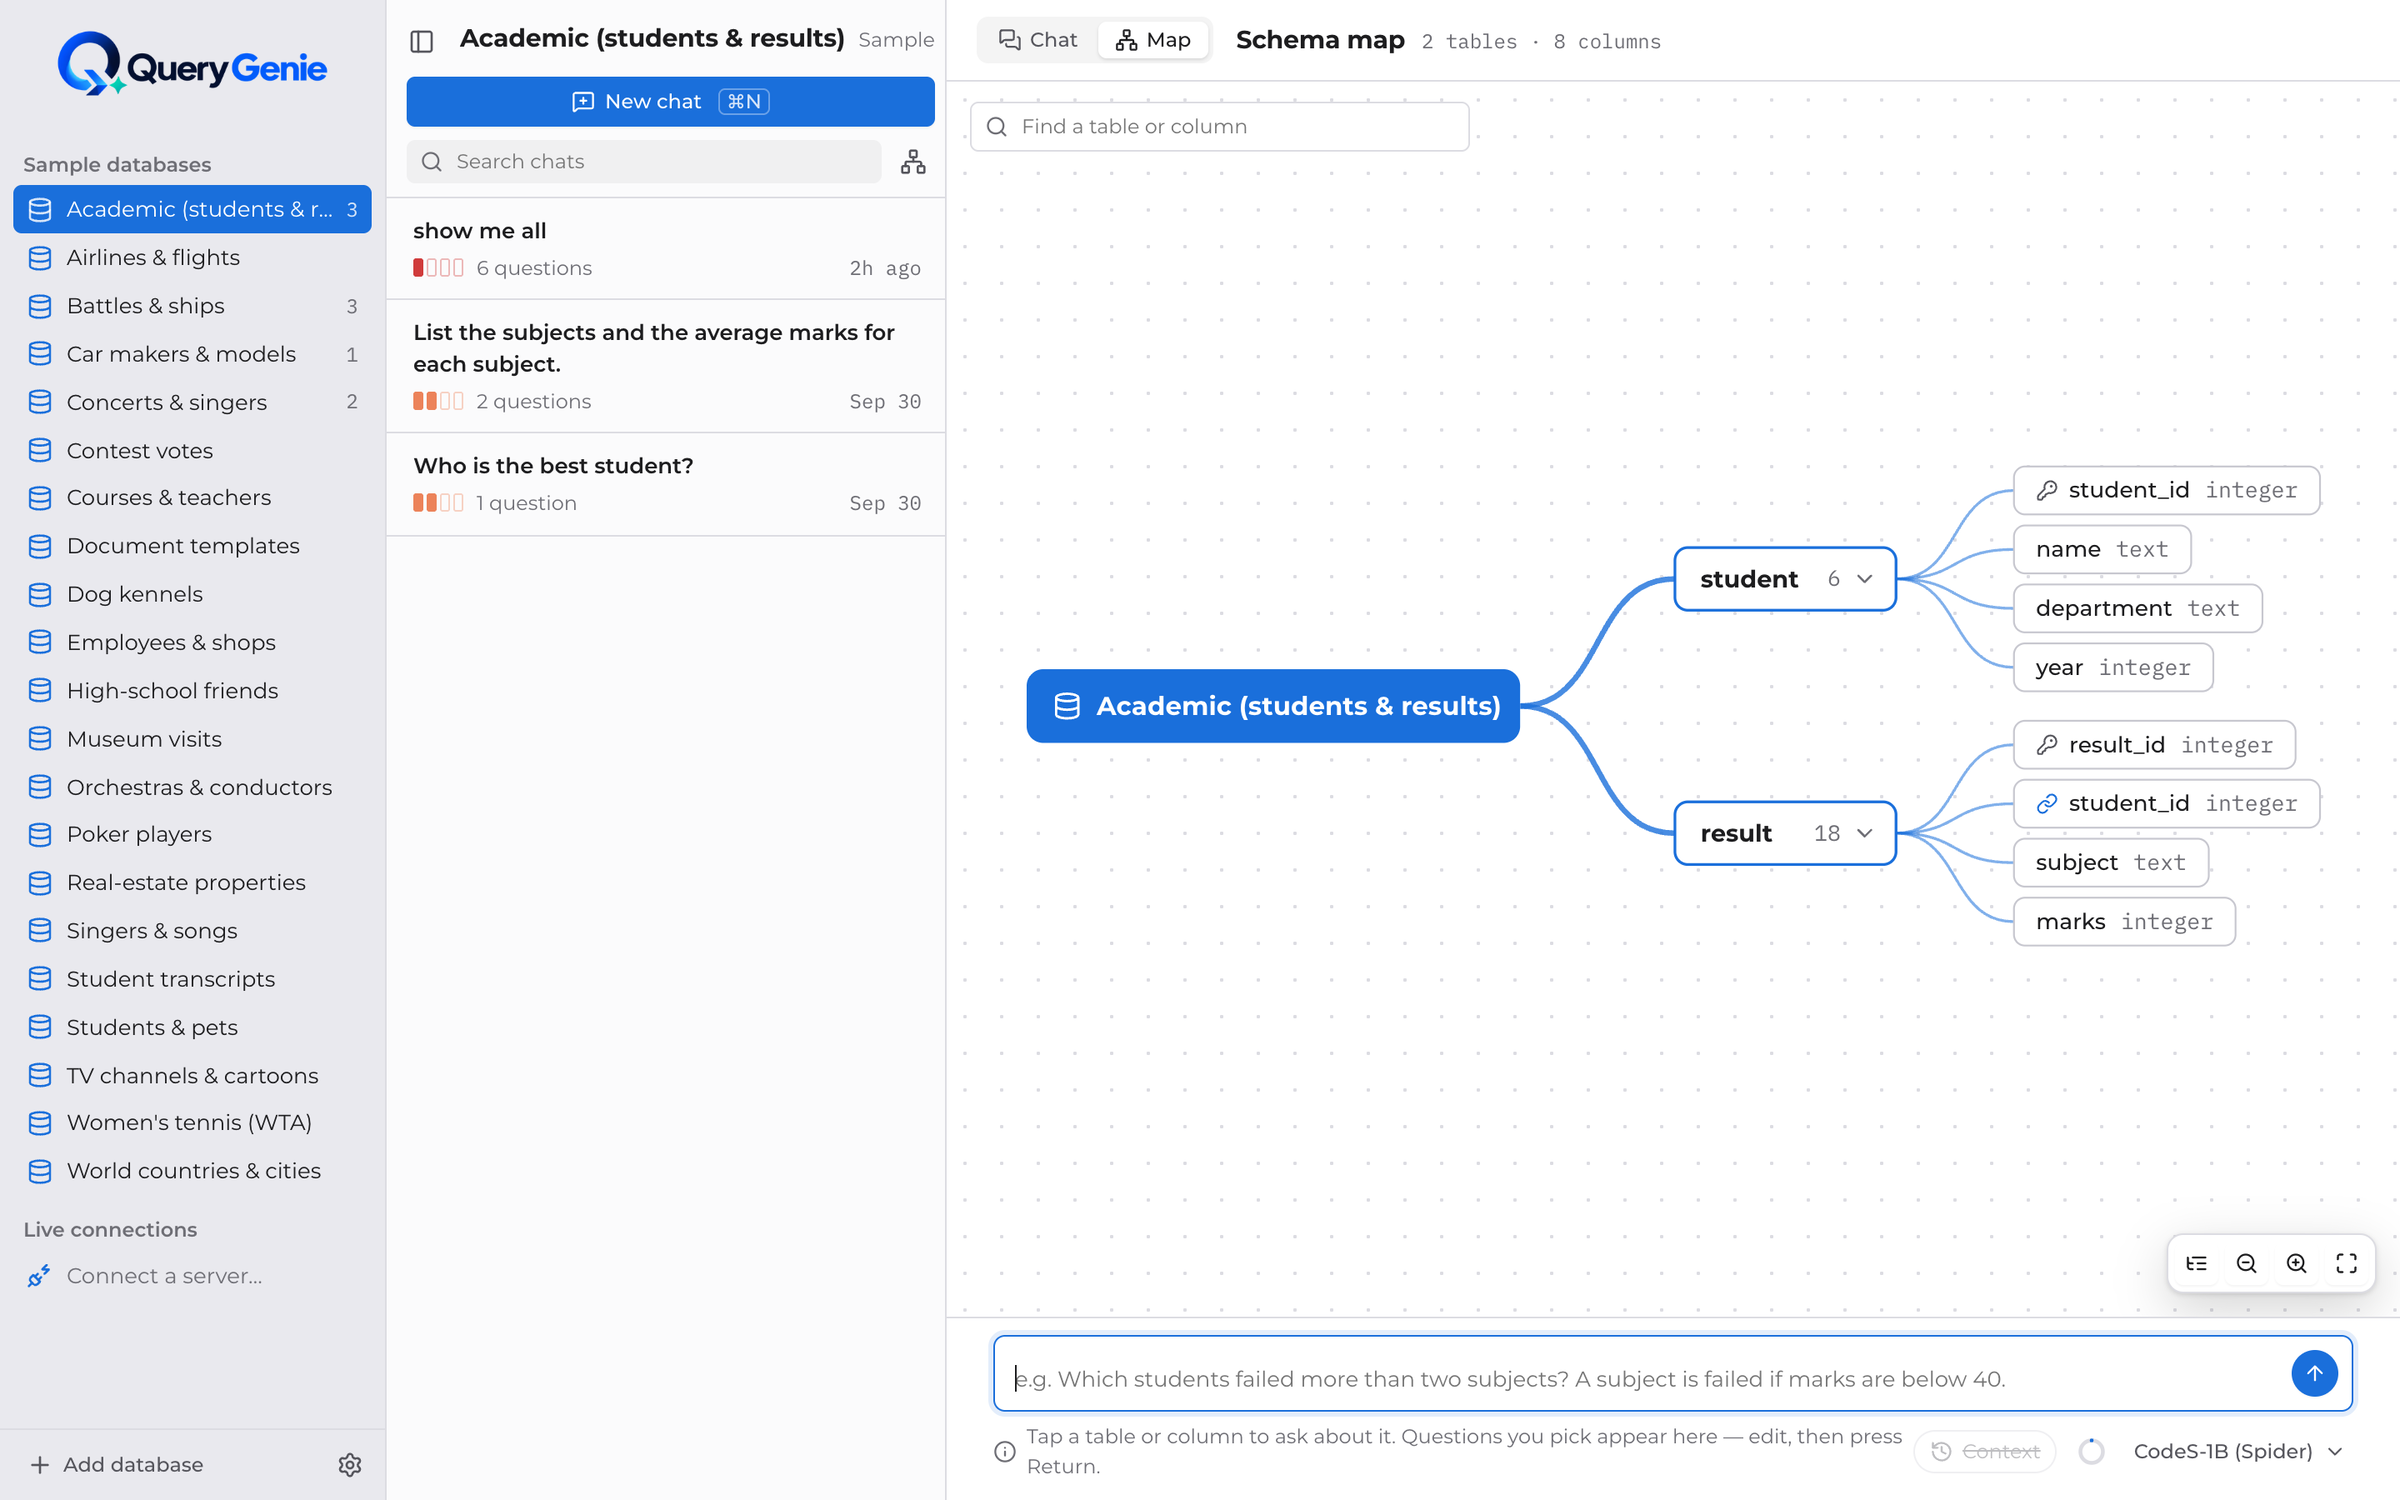
\includegraphics[width=0.49\linewidth]{images/figures/app_schema_map.png}}
	\caption{QueryGenie, the desktop application.}
	\label{fig:app}
\end{figure}
